\documentclass{beamer}
\usepackage{amssymb} % Therefore symbol
\usepackage{hyperref} % URLs
\title{Evaluating risk}
%\subtitle[short]{full}
\author{Andy J. Wills}
\date{}


\begin{document}

\frame{\titlepage}
% Welcome to the last critical thinking lecture of the term. Today, how to evaluate risk.

\begin{frame}{Smoking and risk}
\begin{itemize}
%http://upload.wikimedia.org/wikipedia/commons/3/3b/Smoking_kills.png
\centerline{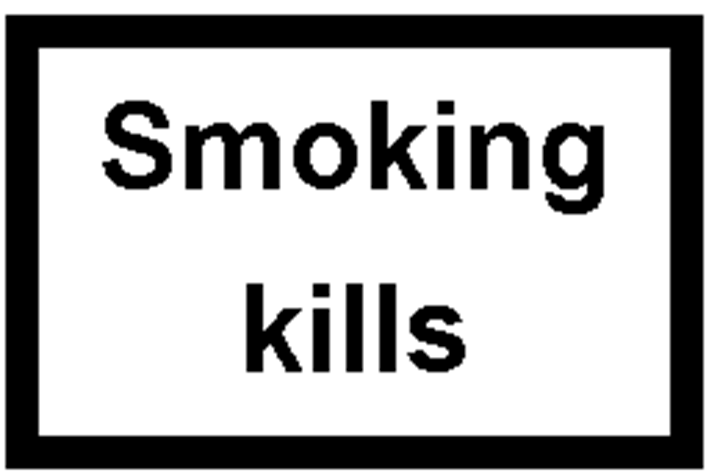
\includegraphics[width=0.5\textwidth]{pics/smokingkills.png}}

\item ``We all gotta die of something''
\item  $P(death|smoker) = 1$
\item  $P(death|nonsmoker) = 1$
\item  How about ``smokers die younger?''

\end{itemize}
\end{frame}

% Let's start with the well-known fag packet warning ``Smoking kills''
% The warning itself - taken literally - must be wrong. It's true that the probability of death,
% given you smoke is 1. The probability of death, given you do not smoke, is also 1. 
% So, your probability of death is unrelated to whether you smoke.
% The daft wording of the warning makes the not uncommon defense:
% ``We all gotta die of something'' entirely reasonable.

\begin{frame}{Smokers die younger (than non-smokers)}
\begin{itemize}
%http://upload.wikimedia.org/wikipedia/commons/thumb/6/64/Cigar_smoking_woman_in_Cuba.jpg/800px-Cigar_smoking_woman_in_Cuba.jpg

\centerline{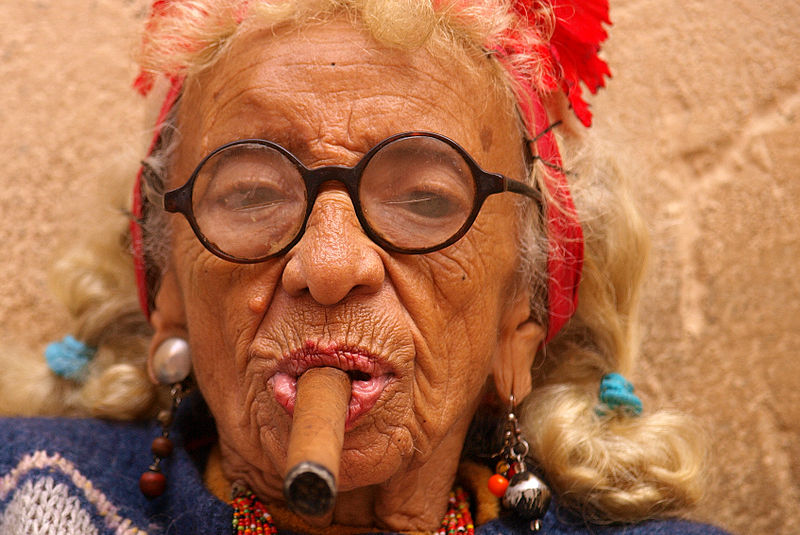
\includegraphics[width=0.5\textwidth]{pics/oldwomansmoking.jpg}}

\item ``I knew a lady who smoked every day, and she lived until she was 93''

\item If the claim is ``ALL smokers die younger than ALL non-smokers''...
\item ...then this counter-example refutes it.
\item Perhaps:
\begin{itemize}
\item ``On average, smokers die younger than non-smokers''
\item ``Smokers have lower life expectancy''
\end{itemize}
\end{itemize}
\end{frame}

% Perhaps a better warning would be ''Smokers die younger [than non-smokers]''

% A not uncommon counter-argument is ``I knew a lady who smoked every day, and she lived until she was 93''

% This counter-argument, although often ridiculed, is also reasonable if one reads the warning as deterministic. In other words, ALL smokers die younger than ALL non-smokers. If that were the argument, the counter-argument would disprove it, because we know lots of people don't make it to 93. 

% The fag packet warning is still ambiguous. What it really means is something like:

% ``On average, smokers die younger than non-smokers'' OR
% ``Smokers have lower life expectancy''

\begin{frame}{Smokers have lower life expectancy}
\begin{itemize}

\item 20\% of smokers die before they are 60 years old 
\item Doll et al.,2004. - Smoking habits of 34000 doctors born 1900-1930.

\item Convinced?
\item Any other information you need?
\end{itemize}
\end{frame}


% OK, how would we go about supporting this clearer claim with data. What if I told you?
% ``20% of smokers die before they are 60''. 
% Are you convinced? What else do you need? 

\begin{frame}{Smokers have lower life expectancy}
\begin{itemize}

\item Think in terms of \emph{hits} and \emph{false alarms}
\item You know $P(DeathBeforeSixty|smoker) = 0.2 $ (hit rate)
\item You also need to know $P(DeathBeforeSixty|nonsmoker)$ (false alarm)
\item $P(DeathBeforeSixty|nonsmoker) = 0.1 $ (Doll et al., 2004)
\end{itemize}
\end{frame}

% What you have is called a hit rate. You also need what's called a ``false alarm'' rate. If 10% of non-smokers die before they are 60, too, then smoking does not affect life expectancy (at least, prior to 60)


\begin{frame}{Odds ratio}
\begin{itemize}

\item $P(DeathBeforeSixty|smoker) = 0.2 $ 
\item $P(DeathBeforeSixty|nonsmoker) = 0.1 $ 
\item Odds ratio, $OR = 0.2 / 0.1 $
\item $OR = 2$
\item Smoking doubles the risk of dying before sixty. 
\end{itemize}
\end{frame}

% ``Yeah, but you could give up smoking and then get hit by a bus''

\begin{frame}{Life is risky}
\begin{itemize}
% http://commons.wikimedia.org/wiki/File:Ljubljana_car_crash_2013.jpg
\centerline{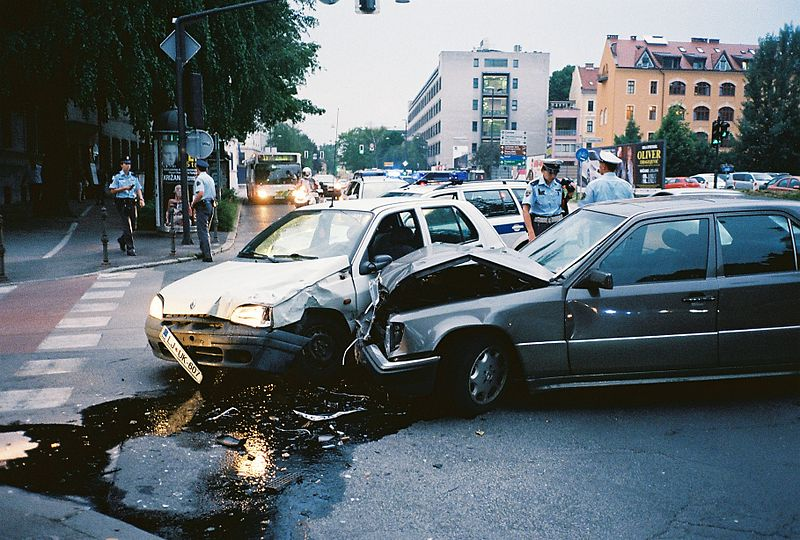
\includegraphics[width=0.5\textwidth]{pics/carcrash.jpg}}
\item ``Yeah, but you could give up smoking and then die in a car accident''
\item ...which possibly means...
\begin{itemize}
\item Many activities have some level of risk.
\item It is impossible to avoid all risk.
\item So everything has to be a risk-benefit analysis otherwise you'd never do anything.
\end{itemize}
\end{itemize}
\end{frame}

% Many activities have some risk. It is impossible to avoid all risk. So everything has to be a risk-benefit analysis otherwise you'd never do anything. 

\begin{frame}{Life is risky? Yes, it is!}
\begin{itemize}
\item Correct. Life is a risk-benefit analysis.
\item Benefit is somewhat subjective - what are the benefits of being a smoker? Or a car driver?
\item ...but odds ratio can help quantify and compare risk.
\end{itemize}
\end{frame}

%http://en.wikipedia.org/wiki/List_of_preventable_causes_of_death
\begin{frame}{Odds ratio}
\begin{itemize}
\item Mokdad et al. (2004) - USA data
\begin{itemize}
\item Tobacco smoking is the cause of death for about 18\% of people.
\item Car accidents are the cause of death for about 0.2\% of people.
\end{itemize}
\item $OR = 18/0.2 = 90$
\item Smoking is 90 times more likely to kill you than driving a car. 
\item Much more than that, actually, because only a minority smoke in the US, but most adults drive regularly.
\end{itemize}
\end{frame}

%http://commons.wikimedia.org/wiki/File:Two_legged_FREAK_(3397831871).jpg
\begin{frame}{I am an individual, not a statistic!}
\centerline{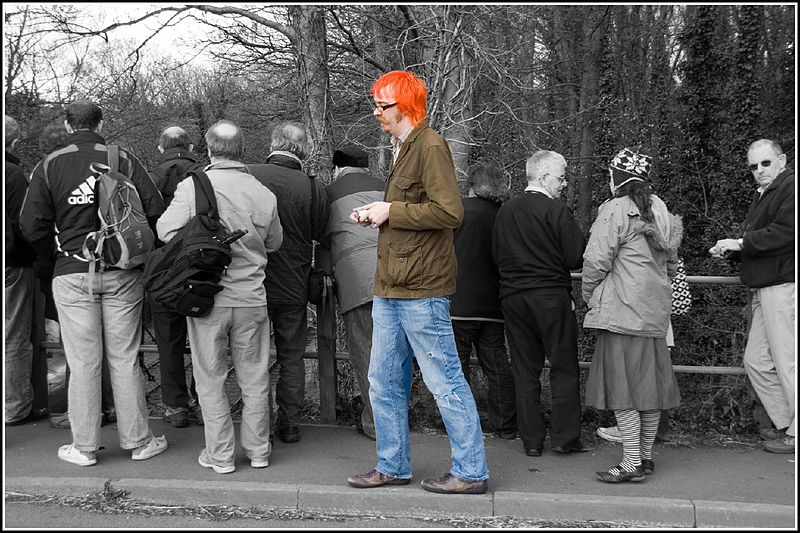
\includegraphics[width=0.5\textwidth]{pics/individual.jpg}}
\begin{itemize}
\item Correct. 
\item These are samples across large numbers of people. They do not \emph{determine} your future cause of death. 
\item But, risk calculations should inform our decisions. Example...
\end{itemize}
\end{frame}

%http://www.telegraph.co.uk/news/9909348/Man-dies-playing-Russian-roulette.html
\begin{frame}{Russian Roulette}
\centerline{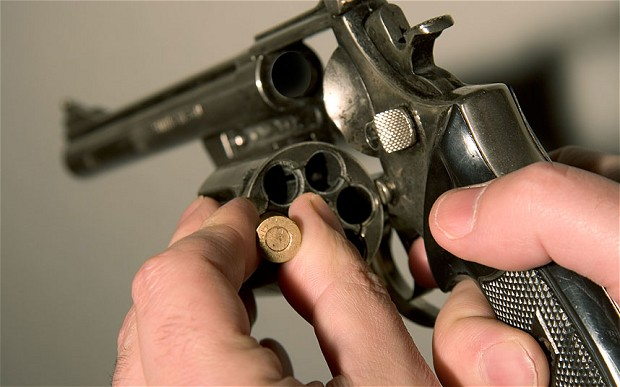
\includegraphics[width=0.5\textwidth]{pics/russianroulette.jpg}}
\begin{itemize}
\item Playing Russian Roulette once, $P(death)= 0.17$
\item After you have played, $P(death) = 1$  or $P(death) = 0$ 
\end{itemize}
\end{frame}

% http://www.flickr.com/photos/terytky/3934371588/sizes/m/in/photostream/
\begin{frame}{Inverse Russian Roulette}
\centerline{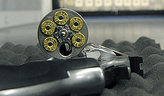
\includegraphics[width=0.5\textwidth]{pics/inverserr.png}}
\begin{itemize}
\item Now imagine \emph{inverse} Russian roulette (five bullets)
\item Playing Inverse Russian Roulette once, $P(death) = .83$
\item Again, after you have played, $P(death) = 1$  or $P(death) = 0$ 
\item If you had to choose between the games, which would you pick ?
\item The odds ratio here is $.83/.17 = 5$ 
\end{itemize}
\end{frame}

% OK, having established that evaluating risk is all about understanding probability, we're going to take a step back and make sure everyone understands the basics of probability.

\begin{frame}{Probability}
\begin{itemize}
\item Probability (by the simplest objective definition) is that property which allows us to calculate the frequency of an event in a very long run of events.

\centerline{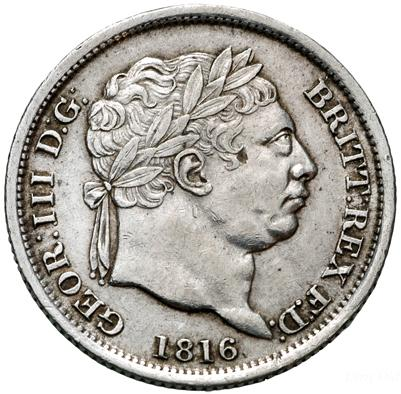
\includegraphics[width=0.2\textwidth]{pics/coin.jpg}}
\item Fair coin 
\begin{itemize}
	\item $P(heads) = 0.5, P(tails) = 0.5$
	\item Flip a fair coin 1000 times, you get close to 500 heads.
	\item The more times you flip the more $heads/flips$ tends towards 0.5.
\end{itemize}
\end{itemize}
\end{frame}

% OK, let's start with the basics. Probability is surprisingly hard to define, but the simplest satisfactory definition is that it allows us to calculate the frequency of an event in a very long run of events.

% So, for example, if I have a fair coin, it can land Heads or Tails, and the probability of each of those events is 0.5. We write this P(heads) = 0.5, P(tails) = 0.5.  If I flip my coin 1,000 times, I would expect to get close to 500 heads. Mathematically: 1000*P(heads) = 1000*0.5 = 500. The more times I flip my coin, the closer the match between the probability and the frequency.

% So, probability of an event is represented P(event) = ..., and the number is always between zero and one.

% As a brief demonstration, estimate the probability of each of these events: 
% Rolling a six on a six-sided dice.
% Having to stand when 60 passengers board a bus with 40 seats.

\begin{frame}{Probability Exercise 1}
\centerline{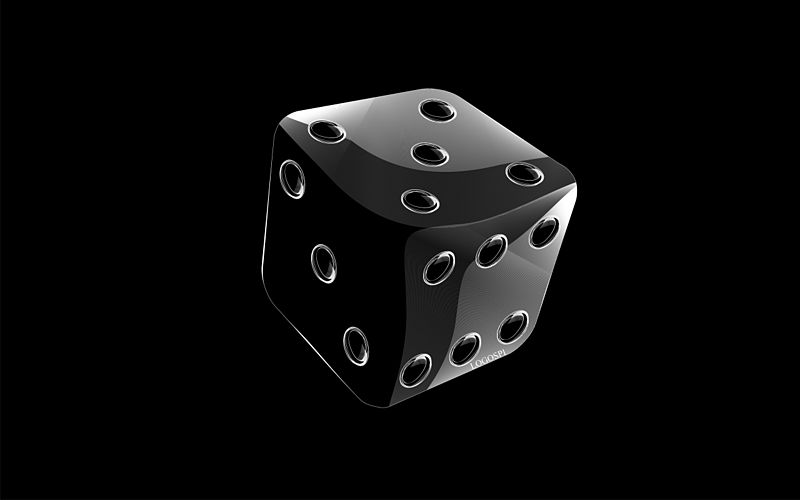
\includegraphics[width=0.4\textwidth]{pics/dice.jpg}}
\begin{itemize}
\item Rolling a six on a six-sided dice.
\item Having to stand when 60 passengers board a bus with 40 seats.
\end{itemize}
\centerline{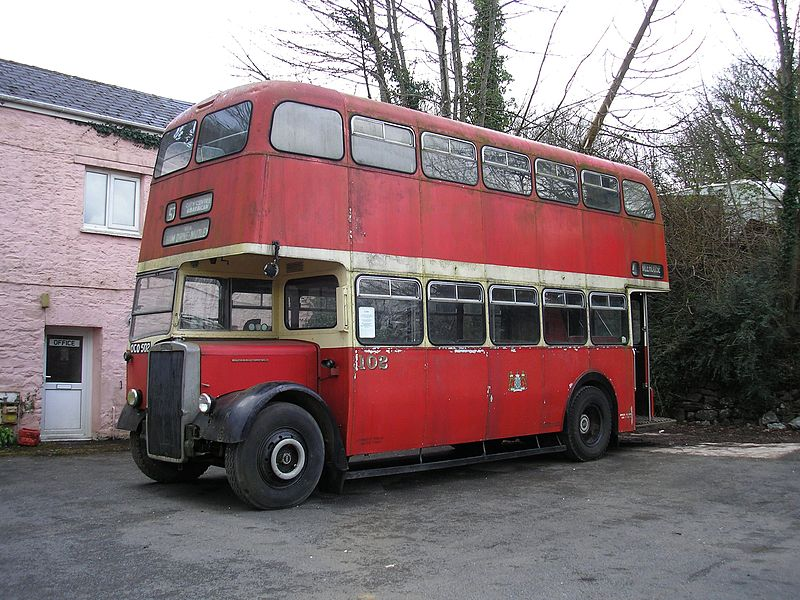
\includegraphics[width=0.4\textwidth]{pics/plymouthbus.jpg}}
\end{frame}

% OK, now how about these:
% Probability of:
% Of dying during 2014, across everyone living in England or Wales (about 0.5%)

% Of getting 4 numbers in the next Lotto game if you buy one ticket (worth around �65). - About 0.1%

% Of committing suicide if you live in England/Wales, are aged 5-34 (about 34% of the population, so about 20 million. About 1000 deaths by suicide in this group - about .005%

\begin{frame}{Probability Exercise 2}
\begin{itemize}
\item Of dying during 2018, across everyone living in England or Wales.
\item Of getting 4 numbers in the next Lotto game if you buy one ticket.
\item Of committing suicide if you live in England/Wales, and are aged 5-34 .
\end{itemize}
\end{frame}

\begin{frame}{GAME SHOW!}
\centerline{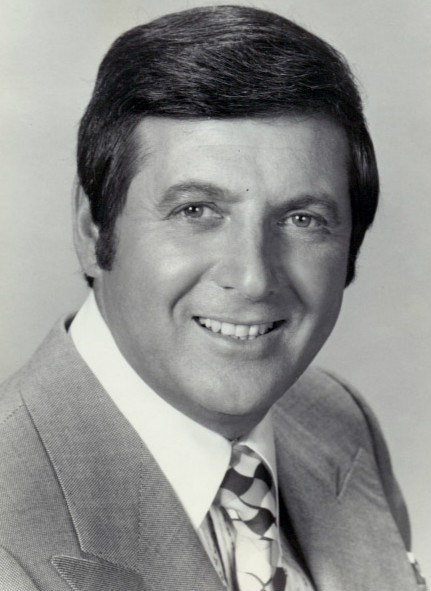
\includegraphics[width=0.3\textwidth]{pics/montyphoto.jpg}}
\centerline{``Let's Make A Deal''}
\centerline{with your host, Monty Hall.}
\end{frame}

\begin{frame}{Monty Hall problem}
\centerline{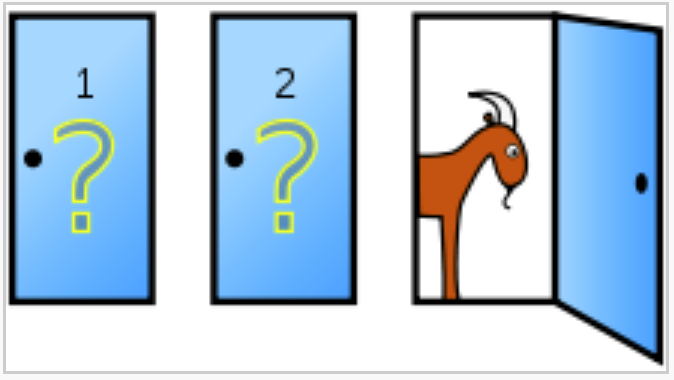
\includegraphics[width=0.5\textwidth]{pics/montyhall.png}}
\begin{itemize}

\item Suppose you're on a game show, and you're given the choice of three doors: Behind one door is a car; behind the others, goats. You want to win the car. You pick a door, say No. 1, and the host, who knows what's behind the doors, opens another door, say No. 3, which has a goat. He then says to you, ``Do you want to pick door No. 2?'' Is it to your advantage to switch your choice? (vos Savant, 1990).
\begin{itemize}
\item Better to switch?
\item Better to stick?
\item Doesn't matter, stick or switch equally likely to win?
\end{itemize}
\end{itemize}
\end{frame}

\begin{frame}{Working out the Monty Hall problem}
\begin{itemize}
\item The host is not going to open the door with the car behind it.
\item On two-thirds of occasions, your first choice will be a goat.
\begin{itemize}
\item The host will then reveal the other goat.
\item So, the car is behind the other door.
\item If you switch, you will win the car
\end{itemize}
\item On one-third of occasions, your first choice will be the car.
\begin{itemize}
\item If you switch, you will not win the car.
\end{itemize}
\item So, on two-thirds of occasions, switching will win the car.
\item You should always switch.
\end{itemize}
\end{frame}

% Statistical independence.

% Basketball players - ask for decisions. (5 min)
% Roulette wheel - ask for decisions. (5 min)

\begin{frame}{Which player would you pass to?}
\centerline{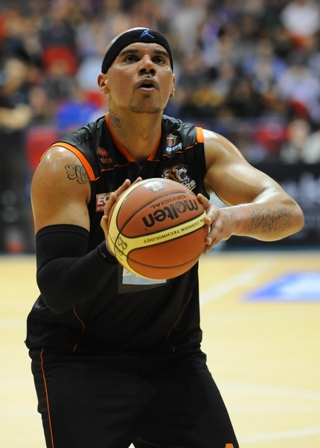
\includegraphics[width=0.4\textwidth]{pics/basketball.jpg}}
\begin{itemize}
\item Player A: Score Score Miss Miss
\item Player B: Miss Miss Score Score
\item A, B, or doesn't matter?
\end{itemize}
\end{frame}

\begin{frame}{Roulette}
\centerline{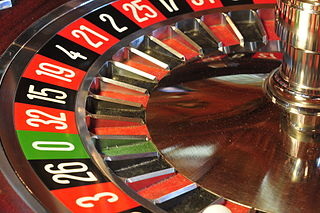
\includegraphics[width=0.8\textwidth]{pics/roulette.jpg}}
\begin{itemize}
\item Red Red Black Red Black Black Black Black 
\item Bet ``red'', bet ``black'', or doesn't matter?
\end{itemize}
\end{frame}

% Roulette Wheel explanation (5 min)
% Basketball player discussion (10 min)

\begin{frame}{Conditional Probability and Randomness}
\begin{itemize}
\item Probability of some event, given that some other event is known to have occurred.
\item $P(heads_{t}|heads_{t-1}) = 0.5$
\item $P(heads_{t}|tails_{t-1}) = 0.5$
\item Events are \textbf{independent} if the conditional probabilities are equal to the unconditional probabilities (as close to an adequate definition of ``random'' as you're ever likely to get).
\item Coin flips, roulette wheels, etc. are demonstrably independent. 
\end{itemize}
\end{frame}

\begin{frame}{Gamblers' fallacy}
\centerline{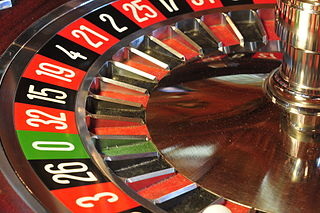
\includegraphics[width=0.4\textwidth]{pics/roulette.jpg}}
\begin{itemize}
\item Red Red Black Red Black Black Black Black 
\item Bet ``red'', bet ``black'', or doesn't matter?
\item Common answer: ``bet red''
\item Rational answers
	\begin{itemize}
		\item If the wheel is known to be unbiased, $P(red) = P(black)$, and it doesn't matter.
		\item From the sample above estimates are that $P(red) < P(black)$, so  bet black.
	\end{itemize}
\end{itemize}
\end{frame}

\begin{frame}{Hot hand fallacy}
\begin{itemize}
\item Player A: Score Score Miss Miss
\item Player B: Miss Miss Score Score
\item A, B, or doesn't matter?
\item Common answer: ``Pass to B'' - Hot Hand fallacy
\item Gilovich, Vallone \& Tversky (1985) - Shots in basketball are independent.
\item Rational answer: Doesn't matter
\item Things to note:
	\begin{itemize}
	\item Basketball experts and players exhibit a hot hand fallacy
	\item Hot Hand and Gamblers' Fallacy are \textbf{opposite} beliefs about independent events. What drives this?
	\end{itemize}
\end{itemize}
\end{frame}

% Interlude (10 min)


% Summary of independence, and a law of probability

\begin{frame}{Independence - Summary}
\begin{itemize}
\item Events are independent if the probabilities conditional on previous events are equal to the unconditional probabilities:
\item For example: $P(heads_{t}|heads_{t-1}) = P(heads_{t}|tails_{t-1}) = P(heads) = 0.5$
\item Failure to understand independence leads to Gamblers' Fallacy and Hot Hand Fallacy.
\end{itemize}
\end{frame}


\begin{frame}{Linda}
\begin{itemize}
\item Linda is 31 years old, single, outspoken, and very bright. She majored in philosophy. As a student, she was deeply concerned with issues of discrimination and social justice, and also participated in anti-nuclear demonstrations.
\item Which is more probable?
\begin{enumerate}
\item Linda is a bank teller.
\item Linda is a feminist bank teller.
\end{enumerate}
\end{itemize}
\end{frame}

\begin{frame}{Conjunction fallacy}
\begin{itemize}
\item Which is more probable?
\begin{enumerate}
\item Linda is a bank teller
\item Linda is a bank teller and is active in the feminist movement.
\end{enumerate}
\item The probability of two events both happening can NEVER be higher than the probability of just one happening. 
\end{itemize}
\end{frame}

\begin{frame}{The conjunction rule}
The probability of two \emph{independent} events both occurring is the product of their individual probabilities.
\begin{itemize}
\item $P(heads_{time 1}) = 0.5$
\item $P(heads_{time 2}) = 0.5$
\item $P(heads_{times 1 and 2}) = P(heads_{time 1}) \times P(heads_{time 2}) = 0.5 \times 0.5 = 0.25$
\item $P(teller) = .05, P(feminist) = .95$
\item $P(teller + feminist) = .05 \times .95 = .0475$
\item $P(teller + feminist) < P(feminist)$
\end{itemize}
\end{frame}

\begin{frame}{Sally Clark}
\centerline{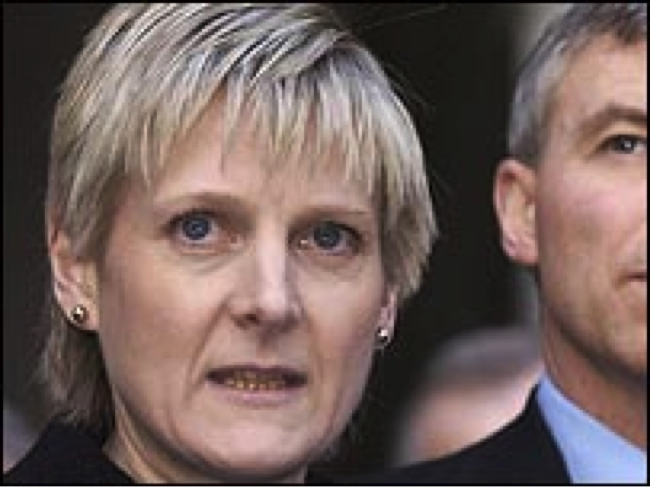
\includegraphics[width=0.5\textwidth]{pics/sallyclark.png}}
\begin{itemize}
\item Solicitor; born 1964.
\item Christopher died at 11 weeks.
\item One year later, Harry died at 8 weeks.
\item Little to no forensic evidence.
\item No evidence she had been a violent or uncaring parent.
\end{itemize}
\end{frame}

\begin{frame}{Roy Meadows}
\centerline{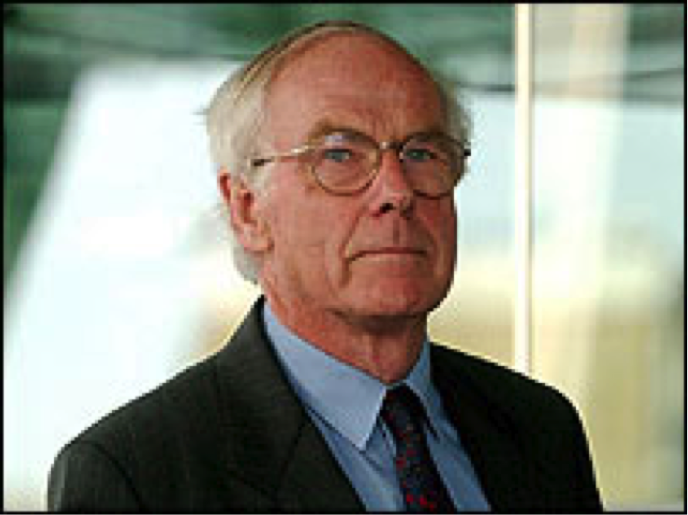
\includegraphics[width=0.5\textwidth]{pics/roymeadows.png}}
\begin{itemize}
\item Sally convicted of murder, spent three years in prison
\item Central to conviction was evidence of expert witness Prof. Roy Meadows:
\begin{itemize}
\item Probability of two cot deaths in the same family was 1 in 73 million
\item Less than once a century in the UK.
\end{itemize}
\item Released on appeal, partly because Prof. Meadows's \textbf{probabilistic inference} was demonstrably wrong.
\end{itemize}
\end{frame}

% Sally Clark; wrong and right statistics. (10 minutes)

\begin{frame}{Roy Meadows - expert witness}
\begin{itemize}
\item Chances of a randomly chosen baby dying of cot death are 1 in 1303, $p = .0008$
\item If the family is affluent, and the mother is over 26, then the chances are even lower; 1 in 8500, $p = .0001$
\item Through the multiplicative law, the probability of two cot deaths in the same family is $ .0001 \times .0001 = 1 \times 10^{-8}$
\item 1 in 73 million
\item Less than once a century in the UK.
\item The idea that these deaths were by natural causes can be ruled out beyond \emph{reasonable doubt}.
\end{itemize}
\end{frame}

\begin{frame}{Roy Meadows - expert witness}
\begin{itemize}
\item Chances of a randomly chosen baby dying of cot death are 1 in 1303, $p = .0008$
\item If the family is affluent, and the mother is over 26, then the chances are even lower; 1 in 8500, $p = .0001$
\item Through the \textbf{multiplicative law}, the probability of two cot deaths in the same family is $ .0001 \times .0001 = 1 \times 10^{-8}$ ... \textbf{COT DEATHS WITHIN THE SAME FAMILY ARE HIGHLY UNLIKELY TO BE INDEPENDENT EVENTS}.
\item 1 in 73 million
\item Less than once a century in the UK.
\item The idea that these deaths were by natural causes can be ruled out beyond \emph{reasonable doubt}.
\end{itemize}
\end{frame}

\begin{frame}{Shared birthdays}
	\begin{itemize} 
		\item In a class of 30 children, what's the probability that there is a shared birthday in the class? (Assume independence, and equiprobability of birth date).
		\item More likely there is, or more likely there is not?
	\end{itemize}
\end{frame}

\begin{frame}{More high-school maths}
\begin{itemize}
\item Number of pairs: $n(n-1)/2$
\item This gets very large quite quickly.
\item Pairs in a group of 2: $2(1)/2 = 1$
\item Pairs in a group of 5: $5(4)/2 = 10$
\item Pairs in a group of 10: $10(9)/2 = 45$
\item Pairs in a group of 20: $20(19)/2 = 190$
\item Pairs of children in a class of 30: $30(29)/2 = 435$
\item Pairs in Year 1 psychology, approx: $300(299)/2 = 44850$
\end{itemize}
\end{frame}

\begin{frame}{Birthday example}
	\begin{itemize} 
		\item 365 days in the year (ignore Feb 29th).
		\item So, the chance of one pair of kids sharing a birthday is $1/365 = .003$
		\item Thus, chance of not sharing is .997
		\item If no pair of kids share a birthday, then there is no shared birthday in the class.
		\item How many pairs in the class?
		\item $n(n-1)/2 = 30 \times 29/2 = 435$.	
		\item Under conjunction rule, $p = .997^{435} = .17$
		\item Thus, probability of a shared birthday is 1-.17 = .83	
	\end{itemize}
\end{frame}

\begin{frame}{Summary}
\begin{itemize}
\item Conjunction rule (Linda)
\item Events are not always independent (Sally Clarke)
\item If a lot of things all have to happen, this is quite unlikely, even if each event is individually very likely (avoiding hurricanes for 100 years; all non-shared birthdays in a class of 30).
\item The number of pairs in a large group is much bigger than you think it is. This can often lead us to make incorrect predictions about large groups. 
\end{itemize}
\end{frame}

% Reading
\begin{frame}{Further Reading}
Helpful background, only lecture content on these topics is examinable).
\begin{itemize}
\item Paulos (1988/2000). \emph{Innumeracy}. Penguin.
\item  \url{http://en.wikipedia.org/wiki/Conjunction_fallacy}
\item  \url{http://en.wikipedia.org/wiki/Sally_Clark}
\item  \url{http://en.wikipedia.org/wiki/Probability}
\end{itemize}
\end{frame}

\end{document}

%%% Local Variables:
%%% mode: latex
%%% TeX-master: t
%%% End:
